
\chapter*{Lecture 36}

\begin{recall}{}{}
\begin{itemize}
\item Power series
\item Project: comments? Latex, useful?
\end{itemize}
\end{recall}

\section{Properties of Power Series}
\subsection{Radius of convergence}
If a power series exists about $x_0$:
\begin{align*}
\sum^\infty_{n=0}a_n(x-x_0)^n=a_0+a_1(x-x_0)+a_2(x-x_0)^2 + \hdots
\end{align*}
where $a_i$ are constants, the power series converges at the point $x=c$ if:
\begin{align*}
\lim_{N\rightarrow\infty}\sum^N_{n=0} a_n(c-x_0)^n
\end{align*}
\textbf{exists.}\\
The number $R$ is called the radius of convergence of the power series such that the series converges absolutely for $\left|x-x_0\right|<R$ and diverges for $\left|x-x_0\right|>R$
\subsection{Computing the radius of convergence}
If for $n$ large, the coefficients $a_n$ are non-zero and satisfy:
\begin{align*}
\lim_{n\rightarrow\infty}\left|\frac{a_n}{a_{n+1}}\right|=L
\end{align*}
then the radius of convergence is $R=L$

\subsection{Shifting the summation index}
The summation index in a power series is a dummy index. In other words, we can change it to suit our needs.
For example, we seek to express the following power series 
\begin{equation*}
\sum^\infty_{n=2}=n(n-1)a_nx^{n-2}
\end{equation*}
in terms of $x^k$ instead of $x^{n-2}$. We can set $k=n-2$ which equals: $n=k+2$ or $n-1=k+1$. Based on this change in dummy variable, $k=0$ when $n=2$. We have:  
\begin{equation*}
\sum^\infty_{n=2}=n(n-1)a_nx^{n-2}=\sum^\infty_{k=0}=(k+2)(k+1)a_{k+2}x^{k}
\end{equation*}


\subsection{Specific properties}
\begin{itemize}
\item Addition and subtraction: If $f(x)=\sum^\infty_{n=0}a_n(x-x_0)^n$ and $g(x)=\sum^\infty_{n=0}b_n(x-x_0)^n$, then $f(x)+g(x)=\sum^\infty_{n=0}(a_n+b_n)(x-x_0)^n$
\item Multiplication: If $f(x) \cdot g(x)=\sum^\infty_{n=0}(c_n)(x-x_0)^n$ where $c_n=\sum^n_{k=0}a_kb_{n-k}$
\item Differentiation: $f'(x)=\sum^\infty_{n=1}n a_n(x-x_0)^{n-1}$ or  $f''(x)=\sum^\infty_{n=2}n(n-1) a_n(x-x_0)^{n-2}$
\item Integration: $\int f(x)=\sum^\infty_{n=0}\frac{a_n}{n+1}(x-x_0)^{n+1}$
\end{itemize}

\section{Power Series Solution to Linear ODEs}

To apply the power series method, given:
\begin{equation*}
p(x)y''+q(x)y'+r(x)y=0
\end{equation*}
$x_0$ needs to be an \textbf{ordinary points} of the ODE. A point $x_0$
is an ordinary point  if $p(x_0) \neq 0$: Otherwise $x_0$ is a singular point. Another way, is to check that given $p(x)=1$, $q(x)$  and $r(x)$ are analytical at $x_0$

\begin{exmp}{}
Find the power series about $x_0=0$ of:
\begin{equation*}
y'+2xy=0
\end{equation*}
\textbf{Solution:}\\
\begin{enumerate}
\item $x_0$ is an ordinary points.
\item Express the solution as a power series:

\begin{align*}
y(x) = \sum^\infty_{n=0} a_n\left(x-x_0\right)^n\\
y'(x) = \sum^\infty_{n=0} a_n n\left(x-x_0\right)^{n-1}
\end{align*}
Since $n=0$, the first term of the series is zero!

\begin{align*}
y'(x) = \sum^\infty_{n=1} a_n n\left(x-x_0\right)^{n-1}
\end{align*}

We can sub into the ODE:
\begin{equation*}
\sum^\infty_{n=1} a_n n\left(x-x_0\right)^{n-1}+2x\sum^\infty_{n=0} a_n\left(x-x_0\right)^n=0
\end{equation*}
Since $x_0=0$:
\begin{equation*}
\sum^\infty_{n=1} a_n nx^{n-1}+\sum^\infty_{n=0} 2a_nx^{n+1}=0 % x needs to be multiplied into the sum to get x^{n+1}
\end{equation*}
\item Apply a "shifting index":
\begin{align*}
let \begin{cases}
k=n-1 \qquad &n=k+1\\
n=1 &k=0\\
n=\infty &k=\infty
\end{cases}
\end{align*}
 and 
 \begin{align*}
let \begin{cases}
j=n+1 \qquad &n=j-1\\
n=0 &j=1\\
n=\infty &j=\infty
\end{cases}
\end{align*}
Our equation becomes:
\begin{equation*}
\sum^\infty_{k=0} a_{k+1} (k+1) x^{k}+\sum^\infty_{j=1}2 a_{j-1}x^{j}=0
\end{equation*}
or:
\begin{equation*}
\sum^\infty_{k=0} a_{k+1} (k+1) x^{k}+\sum^\infty_{k=1}2 a_{k-1}x^{k}=0
\end{equation*}
($k$ and $j$ are indices only!)

We can rewrite as:
\begin{equation*}
a_1x^0+ \sum^\infty_{k=1}\left[ a_{k+1} (k+1)+ 2 a_{k-1}\right]x^{k}=0
\end{equation*}
Since both sides have to be equal, it is clear that:
\begin{align*}
 \begin{cases}
a_1=0\\
a_{k+1}(k+1)+2a_{k-1}=0 \qquad \text{for } k\geq 1
\end{cases}
\end{align*}
or again:
\begin{align*}
a_{k+1}=-\frac{2}{k+1}a_{k-1}
\end{align*}
If $a_0$ is known (via the defined initial conditions), and we know that $a_1=0$ (shown above), $a_n$ can be calculated iteratively.

\begin{tabular}{ l c l l}
k &k+1& $a_{k-1}$     & $a_{k+1}$\\ \hline
1 & 2 & $a_0$         & $a_2 = -\frac{2}{2}a_0=-a_0$\\ 
2 & 3 & $a_1=0$       & $a_3=-\frac{2}{3} a_1=0$ \\
3 & 4 & $a_2=-a_0$    & $a_4=-\frac{2}{4} a_2=\frac{1}{2}a_0$ \\
4 & 5 & $a_3=0$       & $a_5=-\frac{2}{5} a_3=0$ \\
5 & 6 & $a_4 =\frac{1}{2}a_0$ & $a_6=-\frac{2}{6} a_4=-\frac{1}{6}a_0 =\frac{1}{3!}a_0 $ \\
\end{tabular}
The solution becomes:
\begin{align*}
y(x)=a_0-a_0x^2+\frac{a_0}{2!}x^4-\frac{a_0}{3!}x^6+\frac{a_0}{4!}x^8 +\hdots= a_0\sum^\infty_{n=0}\frac{(-1)^n}{n!}x^{2n}
\end{align*}
The exact solution is:
\begin{align*}
y(x)=a_0e^{-x^2}
\end{align*}
where $a_0$ is determined by the initial condition (not given in this problem).
\begin{figure}[h!]
\centering
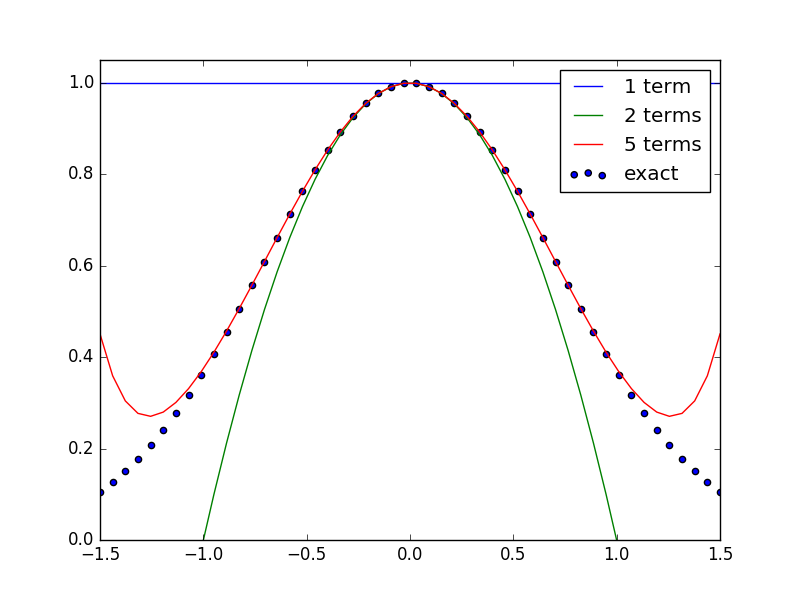
\includegraphics[width=\textwidth]{figs/powerSeries.png}
\caption{Evaluation of truncation error of the power series.}
\end{figure}
\end{enumerate}
\end{exmp}

\begin{figure}[h!]
\centering
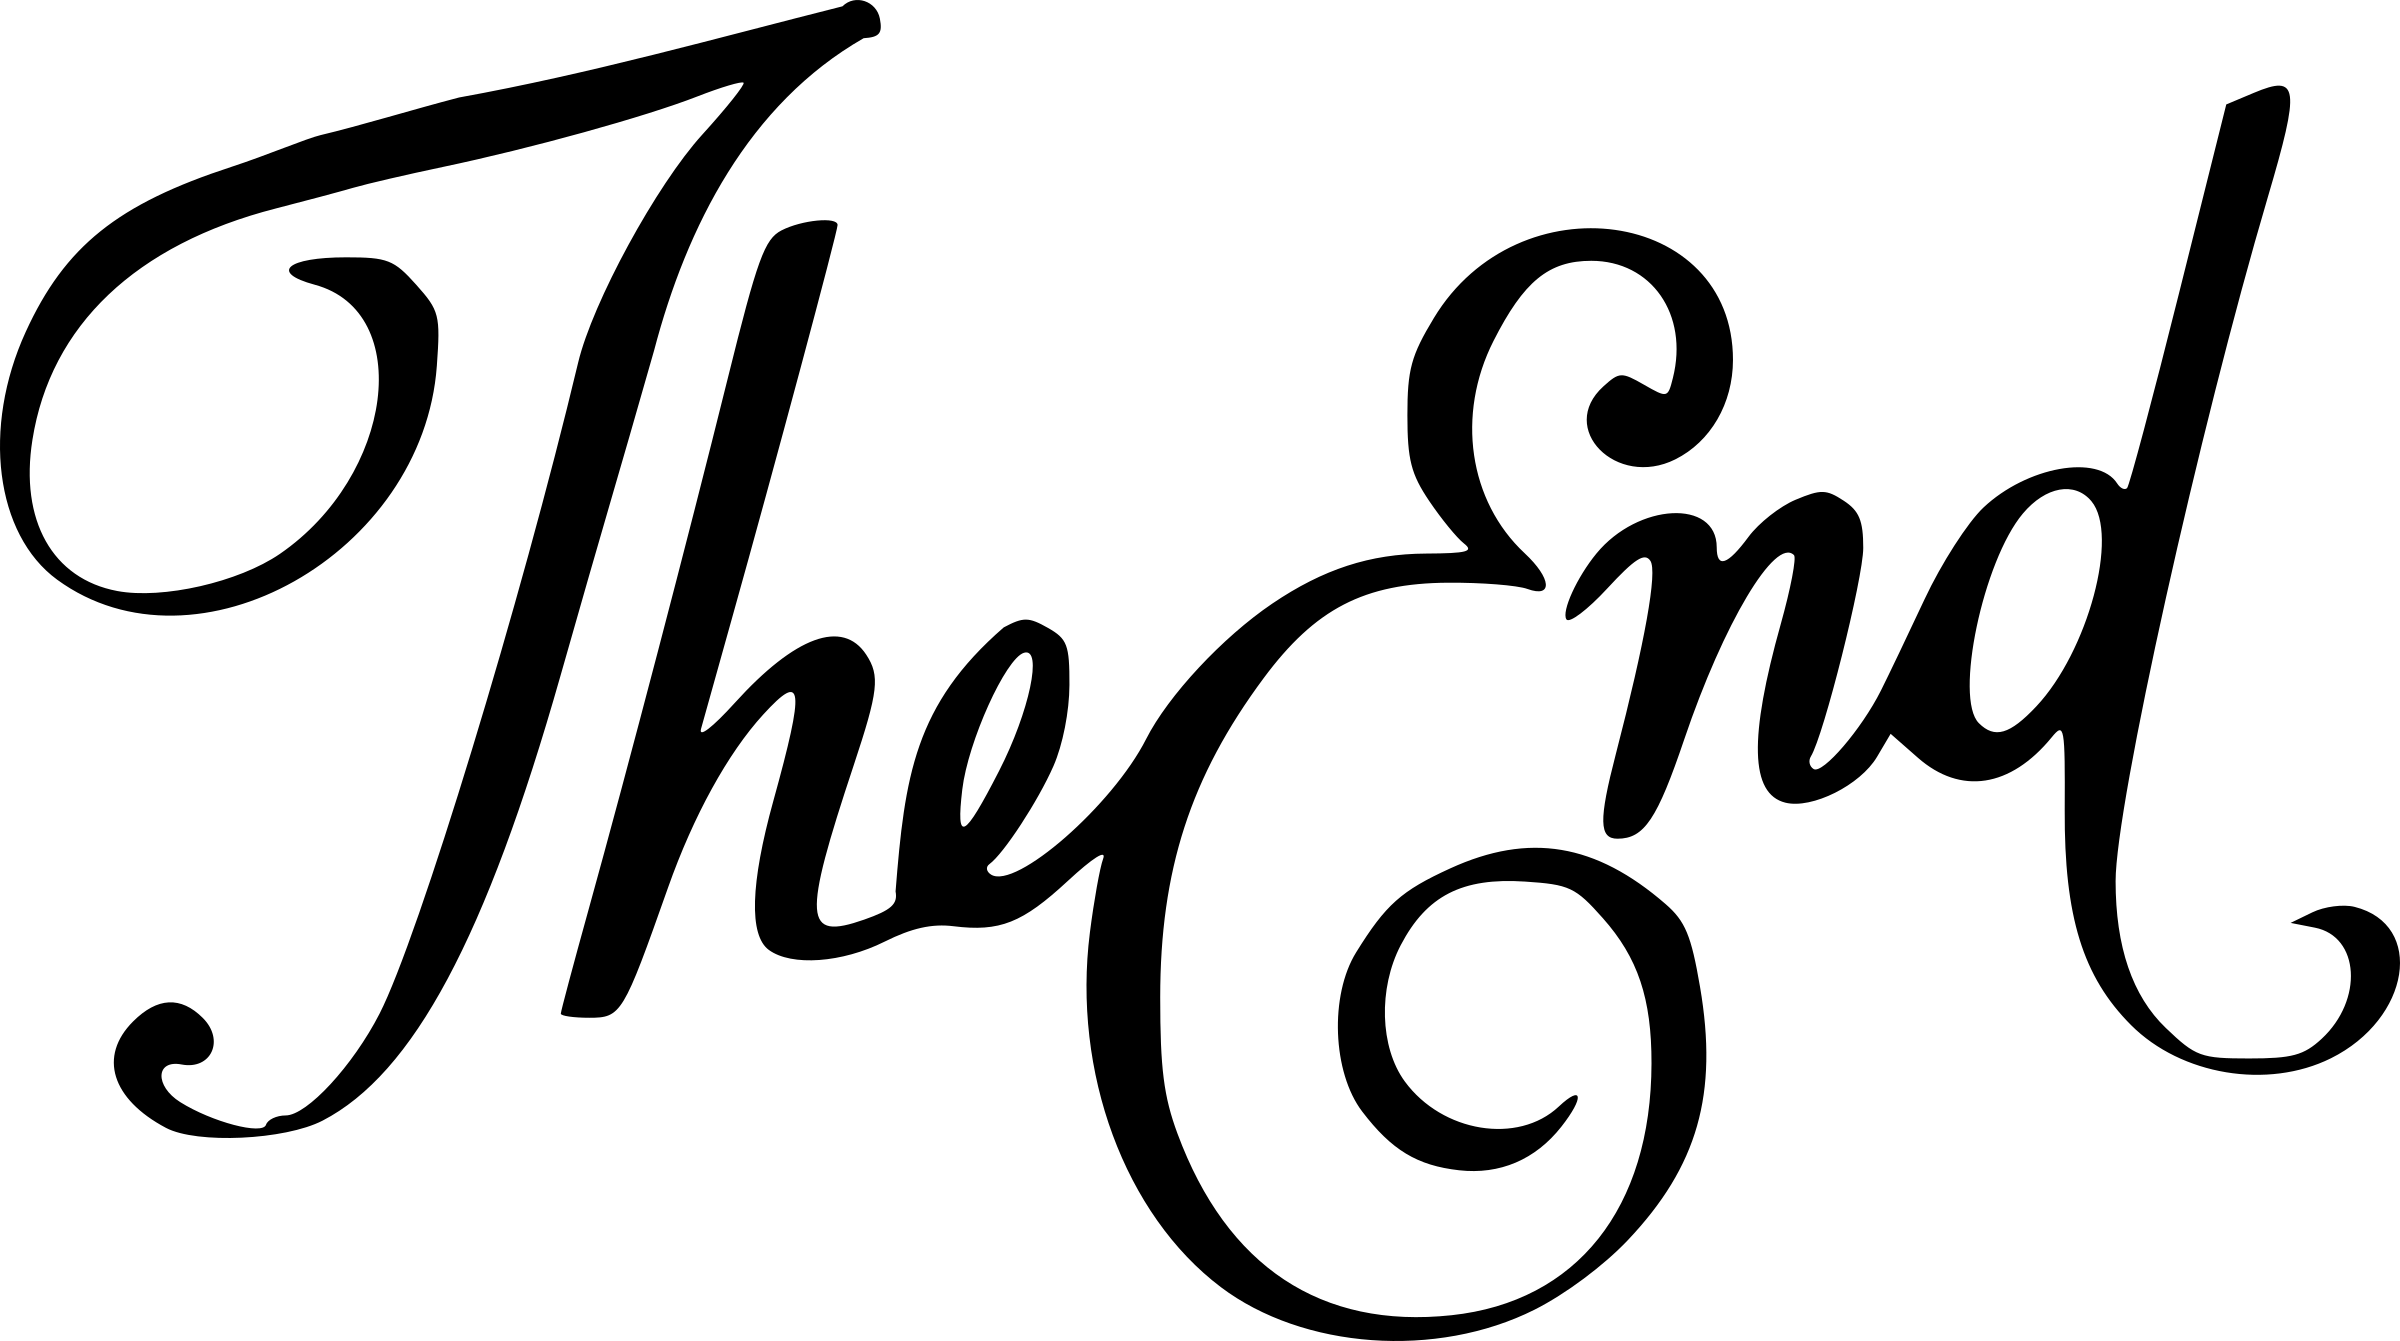
\includegraphics{figs/the_end.png}
\end{figure}

\clearpage


\section*{Course wrap-up}
\subsection*{Course Outcomes:}
\begin{itemize}
\item Classify the resulting differential equations and determine appropriate solution methods for each type
 \item  Apply analytical techniques to solve various differential equations and systems.
\item Formulate mathematical models representing the behaviour of simplified engineering systems.  
 \end{itemize}

\subsection*{Exam preparation}
The final exam will cover all the material seen in class, tutorial, and assignments (except the finite difference discussion last lecture). A strong emphasis will be placed on the material learned since the mid-term. That said, important concepts from the pre mid-term may still be asked. The weighting of the concepts will be propotional to the number of class hours (post mid-term).

\subsection*{Tips for preparation}
\begin{itemize}
\item Understand the theory in the class notes and book
\item Do practice exams (many universities have sample exams online)
\item Complete all of the assignments
\item Review all of the tutorial problems
\item (if time permits) do problems from other textbooks
\end{itemize}



\subsection*{Exam questions}
(The grade distribution is approximative!)
\begin{itemize}
\item Will contain multiple choice questions (about 10-20\% of points)
\item About 40-50\% of the questions will be very similar to the assignments (easy to pick up points)
\item Conceptual questions (about 10-30\%) will evaluate your understanding of the material
\item Mathematical modelling will likely be present (10-30\%)
\end{itemize}


\subsection*{Exam strategy}
\begin{itemize}
\item Carefully use your time for the exam; if you get stuck, pass and come-back.
\item Do not too heavily rely on the formula sheet
\item Partial points are easy to get for the assignment type problems; conceptual problems are more severely graded.
\item  Do not leave the multiple choices empty! You have a chance of getting it right!
\item Final is worth 55\% of the class grade
\end{itemize}

\textbf{Would be happy to get comments on the improvements that could be brought to MTE202 (projects, tutorial, lectures etc.)}


